%% ============================================================
%% From Telemetry to Tests: Building Agentic QA Loops
%% with MCP and Playwright
%% WMF 2026 - Ludovico Besana
%%
%% Compile with:
%%   pdflatex talk.tex
%%   pdflatex talk.tex   (run twice for ToC / overlays)
%%
%% Requirements: TeX Live 2020+ or MiKTeX with beamer,
%%   metropolis, listings, fontawesome5, tikz, booktabs
%% ============================================================

\documentclass[aspectratio=169,10pt]{beamer}

%% ── Theme ────────────────────────────────────────────────────
\usetheme{metropolis}
\usepackage{appendixnumberbeamer}

%% ── Packages ─────────────────────────────────────────────────
\usepackage[utf8]{inputenc}
\usepackage[T1]{fontenc}
\usepackage{booktabs}
\usepackage{xspace}
\usepackage{listings}
\usepackage{tikz}
\usetikzlibrary{arrows.meta, positioning, shapes.geometric, fit, backgrounds, calc}

%% fontawesome5 is optional - comment out if unavailable
\usepackage{fontawesome5}

%% ── Palette (from checkout app CSS) ──────────────────────────
\definecolor{docblue}{HTML}{124e66}
\definecolor{docgreen}{HTML}{116149}
\definecolor{doclightbg}{HTML}{f5efe6}
\definecolor{docmuted}{HTML}{66707b}
\definecolor{codebg}{HTML}{1e1e2e}
\definecolor{codestring}{HTML}{a6e3a1}
\definecolor{codekw}{HTML}{89b4fa}
\definecolor{codecomment}{HTML}{6c7086}
\definecolor{codenumber}{HTML}{fab387}

%% Apply palette to metropolis
\setbeamercolor{normal text}{fg=black!87, bg=white}
\setbeamercolor{frametitle}{bg=docblue, fg=white}
\setbeamercolor{progress bar}{fg=docgreen, bg=docblue!30}
\setbeamercolor{title separator}{fg=docgreen}
\setbeamercolor{alerted text}{fg=docblue}
\setbeamercolor{example text}{fg=docgreen}
\setbeamercolor{block title}{bg=docblue!10, fg=docblue}
\setbeamercolor{block body}{bg=docblue!5}
\setbeamercolor{block title alerted}{bg=red!10, fg=red!70!black}
\setbeamercolor{block body alerted}{bg=red!5}
\setbeamercolor{block title example}{bg=docgreen!10, fg=docgreen}
\setbeamercolor{block body example}{bg=docgreen!5}

%% ── Code listings ────────────────────────────────────────────
\lstdefinestyle{dark}{
  backgroundcolor=\color{codebg},
  basicstyle=\ttfamily\tiny\color{white!90},
  keywordstyle=\color{codekw}\bfseries,
  stringstyle=\color{codestring},
  commentstyle=\color{codecomment}\itshape,
  numberstyle=\tiny\color{codenumber},
  breakatwhitespace=false,
  breaklines=true,
  keepspaces=true,
  showstringspaces=false,
  tabsize=2,
  frame=single,
  framerule=0pt,
  rulecolor=\color{codebg},
  xleftmargin=8pt,
  xrightmargin=4pt,
  aboveskip=4pt,
  belowskip=2pt,
}

\lstdefinelanguage{TypeScript}{
  morekeywords={const,let,var,function,async,await,return,import,from,export,
                test,expect,describe,type,interface},
  sensitive=true,
  morestring=[b]',
  morestring=[b]",
  morestring=[b]`,
  morecomment=[l]{//},
  morecomment=[s]{/*}{*/},
}

\lstdefinelanguage{JSON}{
  morestring=[b]",
  literate=
    *{0}{{{\color{codenumber}0}}}{1}
     {1}{{{\color{codenumber}1}}}{1}
     {2}{{{\color{codenumber}2}}}{1}
     {3}{{{\color{codenumber}3}}}{1}
     {4}{{{\color{codenumber}4}}}{1}
     {5}{{{\color{codenumber}5}}}{1}
     {true}{{{\color{codekw}true}}}{4}
     {false}{{{\color{codekw}false}}}{5}
}

%% ── Metadata ─────────────────────────────────────────────────
\title{From Telemetry to Tests}
\subtitle{Building Agentic QA Loops with MCP and Playwright}
\author{Ludovico Besana}
\date{WMF 2026}
\institute{}

%% ── Helper macros ────────────────────────────────────────────
\newcommand{\cmdbox}[1]{%
  \colorbox{docblue!10}{\texttt{\small\color{docblue}#1}}%
}
\newcommand{\agentbadge}[2]{%
  \colorbox{#1!15}{\small\color{#1!80!black}\textbf{#2}}%
}

%% ─────────────────────────────────────────────────────────────
\begin{document}
%% ─────────────────────────────────────────────────────────────

%% ── Title ────────────────────────────────────────────────────
{
\setbeamercolor{background canvas}{bg=docblue}
\setbeamercolor{normal text}{fg=white}
\begin{frame}[plain]
  \vspace{1.6cm}
  {\color{white}\Huge\bfseries From Telemetry to Tests}\\[0.4em]
  {\color{white!75}\large Building Agentic QA Loops\\with MCP and Playwright}\\[2em]
  {\color{white!60}\normalsize Ludovico Besana \quad\textperiodcentered{}\quad WMF 2026}
\end{frame}
}

%% ── Agenda ───────────────────────────────────────────────────
\begin{frame}{Today's Agenda}
  \begin{columns}[T]
    \column{0.5\textwidth}
      \textbf{\color{docblue}01 \quad The Problem}\\[0.3em]
      \small Why static test suites fail under production pressure

      \vspace{1em}
      \textbf{\color{docblue}02 \quad The Architecture}\\[0.3em]
      \small MCP, three agents, and the data flow

    \column{0.5\textwidth}
      \textbf{\color{docblue}03 \quad Live Demo}\\[0.3em]
      \small From a Grafana spike to a passing Playwright test

      \vspace{1em}
      \textbf{\color{docblue}04 \quad The Bigger Picture}\\[0.3em]
      \small QA engineers as orchestrators of quality systems
  \end{columns}
\end{frame}

%% ══════════════════════════════════════════════════════════════
\section{01 \quad The Problem}
%% ══════════════════════════════════════════════════════════════

\begin{frame}{The Status Quo}
  \begin{columns}[T]
    \column{0.48\textwidth}
      \textbf{How most teams write E2E tests today}

      \vspace{0.6em}
      \begin{itemize}
        \setlength\itemsep{0.5em}
        \item Static suites written once, maintained by hand
        \item AI tools generate a test - you copy-paste it in
        \item Tests are blind to production signals
        \item Failures are discovered on CI, not from user behavior
        \item Flaky tests are silenced with \texttt{.skip}
      \end{itemize}

    \column{0.48\textwidth}
      \begin{alertblock}{The result}
        A growing gap between what observability tells you\\
        and what your test suite is actually testing.
      \end{alertblock}

      \vspace{0.8em}
      Production fires a 27\% checkout error rate at 09:14.\\[0.4em]
      Your test suite has no record of \texttt{/checkout} ever returning 500.
  \end{columns}
\end{frame}

\begin{frame}[fragile]{The Observability Data You Already Have}
  \begin{columns}[T]
    \column{0.52\textwidth}
      Your APM stack captures this on every failed checkout:

      \vspace{0.5em}
      \lstset{style=dark, language=JSON}
      \begin{lstlisting}
{
  "event": "checkout_submit_failed",
  "message": "API returned 500 on /checkout",
  "httpStatus": 500,
  "latencyMs": 1428,
  "k6": {
    "errorRate": 0.27,
    "checks": {
      "submit button visible": true,
      "checkout 2xx": false
    }
  }
}
      \end{lstlisting}

    \column{0.44\textwidth}
      \textbf{What this tells a QA engineer:}

      \vspace{0.6em}
      \begin{itemize}
        \setlength\itemsep{0.5em}
        \item The submit button rendered fine
        \item The \texttt{/checkout} API failed
        \item 1 in 4 submissions affected
        \item The form flow up to the click works
        \item We need a test for the post-submit path
      \end{itemize}

      \vspace{0.8em}
      \begin{exampleblock}{The opportunity}
        This JSON is rich enough to drive test generation - if you have an agent that knows how to read it.
      \end{exampleblock}
  \end{columns}
\end{frame}

\begin{frame}{The Gap We Are Closing}
  \centering
  \resizebox{0.92\textwidth}{!}{%
    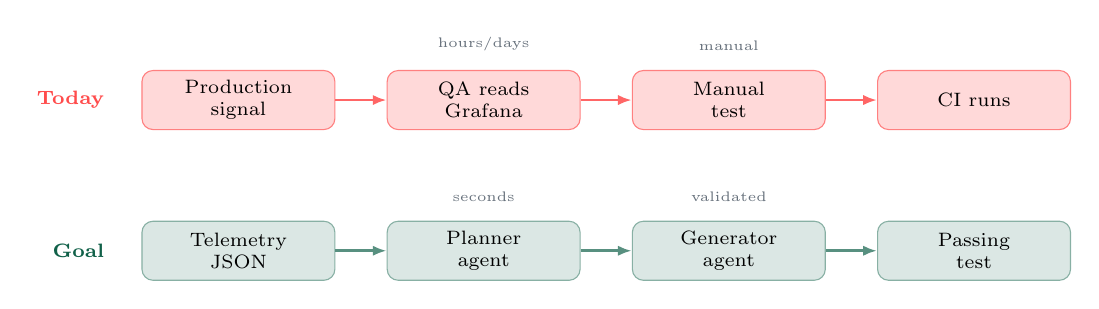
\begin{tikzpicture}[
      box/.style={
        rectangle,
        rounded corners=4pt,
        minimum width=2.45cm,
        minimum height=0.75cm,
        align=center,
        font=\scriptsize
      },
      arr/.style={-{Latex[length=5pt]}, line width=1pt},
      today/.style={box, fill=red!15, draw=red!50},
      target/.style={box, fill=docgreen!15, draw=docgreen!50},
      note/.style={font=\tiny\color{docmuted}}
    ]
      \node[today] (prod) {Production\\signal};
      \node[today, right=0.65cm of prod] (eng) {QA reads\\Grafana};
      \node[today, right=0.65cm of eng] (writes) {Manual\\test};
      \node[today, right=0.65cm of writes] (ci) {CI runs};

      \draw[arr, red!60] (prod) -- (eng);
      \draw[arr, red!60] (eng) -- (writes);
      \draw[arr, red!60] (writes) -- (ci);

      \node[note, above=0.12cm of eng] {hours/days};
      \node[note, above=0.12cm of writes] {manual};

      \node[target, below=1.15cm of prod] (sig) {Telemetry\\JSON};
      \node[target, right=0.65cm of sig] (plan) {Planner\\agent};
      \node[target, right=0.65cm of plan] (gen) {Generator\\agent};
      \node[target, right=0.65cm of gen] (test) {Passing\\test};

      \draw[arr, docgreen!70] (sig) -- (plan);
      \draw[arr, docgreen!70] (plan) -- (gen);
      \draw[arr, docgreen!70] (gen) -- (test);

      \node[note, above=0.12cm of plan] {seconds};
      \node[note, above=0.12cm of gen] {validated};

      \node[
        left=0.35cm of prod,
        font=\scriptsize\bfseries\color{red!70}
      ] {Today};

      \node[
        left=0.35cm of sig,
        font=\scriptsize\bfseries\color{docgreen}
      ] {Goal};
    \end{tikzpicture}%
  }
\end{frame}

%% ══════════════════════════════════════════════════════════════
\section{02 \quad The Architecture}
%% ══════════════════════════════════════════════════════════════

\begin{frame}{Model Context Protocol (MCP)}
  \begin{columns}[T]
    \column{0.48\textwidth}
      \textbf{What MCP is}

      \vspace{0.5em}
      An open protocol that lets LLMs connect to external tools, files, and environments as first-class capabilities - not just text in a prompt.

      \vspace{0.8em}
      \textbf{What it enables here}

      \vspace{0.5em}
      \begin{itemize}
        \setlength\itemsep{0.4em}
        \item Agents read local files directly
        \item Agents run terminal commands
        \item Agents inspect the live browser DOM
        \item Agents write back into the project
      \end{itemize}

    \column{0.48\textwidth}
      \textbf{Without MCP}

      \vspace{0.4em}
      \small "Here is the telemetry JSON and the seed test.
      Write me a test." (paste, copy, paste again)

      \vspace{0.8em}
      \textbf{With MCP}

      \vspace{0.4em}
      \small The agent reads the telemetry, opens the browser,
      validates selectors, and writes the test file - in one
      uninterrupted action loop.

      \vspace{0.8em}
      \begin{exampleblock}{}
        MCP is the connective tissue that turns an LLM into an agent that acts in your project.
      \end{exampleblock}
  \end{columns}
\end{frame}

\begin{frame}{The Three-Agent Loop}
  \begin{center}
    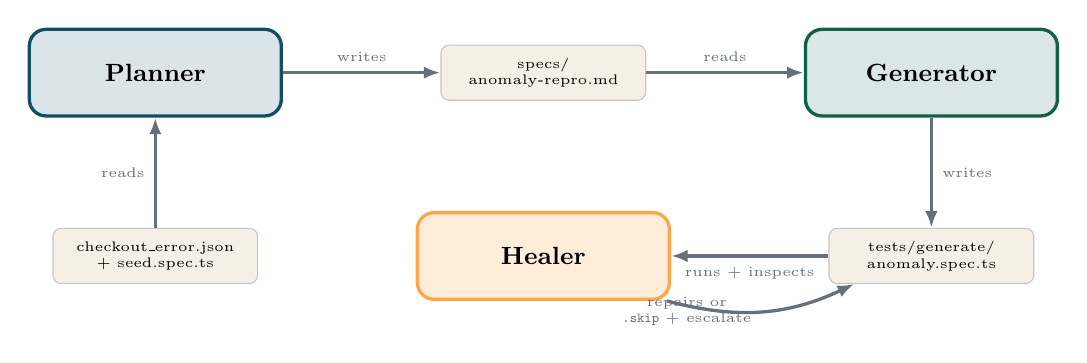
\begin{tikzpicture}[
      agent/.style={rectangle, rounded corners=6pt, minimum width=3.2cm,
                    minimum height=1.1cm, align=center, font=\small\bfseries,
                    line width=1.2pt},
      file/.style={rectangle, rounded corners=3pt, minimum width=2.6cm,
                   minimum height=0.7cm, align=center, font=\tiny,
                   fill=doclightbg, draw=docmuted!40},
      arr/.style={-{Latex[length=6pt]}, line width=1.2pt, color=docmuted},
      label/.style={font=\tiny\color{docmuted}, align=center},
    ]
      \node[agent, fill=docblue!15, draw=docblue] (planner) {Planner};
      \node[file, right=2.0cm of planner] (spec) {specs/\\anomaly-repro.md};
      \node[agent, fill=docgreen!15, draw=docgreen, right=2.0cm of spec] (gen)
            {Generator};
      \node[file, below=1.4cm of gen] (test) {tests/generate/\\anomaly.spec.ts};
      \node[agent, fill=orange!15, draw=orange!70, left=2.0cm of test] (healer)
            {Healer};
      \node[file, below=1.4cm of planner] (telem) {checkout\_error.json\\+ seed.spec.ts};

      \draw[arr] (telem) -- (planner) node[midway,left,label]{reads};
      \draw[arr] (planner) -- (spec) node[midway,above,label]{writes};
      \draw[arr] (spec) -- (gen) node[midway,above,label]{reads};
      \draw[arr] (gen) -- (test) node[midway,right,label]{writes};
      \draw[arr] (test) -- (healer) node[midway,below,label]{runs + inspects};
      \draw[arr] (healer) to[bend right=20]
                 node[midway,left,label]{repairs or\\\texttt{.skip} + escalate} (test);
    \end{tikzpicture}
  \end{center}
\end{frame}

\begin{frame}[fragile]{Agent 1: The Planner}
  \begin{columns}[T]
    \column{0.42\textwidth}
      \agentbadge{docblue}{Planner}

      \vspace{0.6em}
      \textbf{Input}\\
      Telemetry JSON + grounded seed test

      \vspace{0.6em}
      \textbf{Output}\\
      \texttt{specs/anomaly-repro.md}

      \vspace{0.6em}
      \textbf{Guardrail}\\
      Verifies every selector exists in the live DOM. If a required flow is absent, escalates - does not hallucinate a plan.

      \vspace{0.6em}
      \textbf{Claude Code command}\\
      \cmdbox{/plan}

    \column{0.54\textwidth}
      Spec output shape:
      \lstset{style=dark}
      \begin{lstlisting}[language={}]
# Anomaly Reproduction: Checkout Error

## Intent
Reproduce the HTTP 500 spike on /checkout.

## Steps
1. Open the checkout page
2. Confirm session banner shows Ada Lovelace
3. Fill shipping name, email, address, postal
4. Select Standard shipping
5. Select Credit Card payment
6. Click Submit payment

## Selector Map
shipping-form:    [data-testid="shipping-form"]
payment-button:   [data-testid="payment-button"]
checkout-message: [data-testid="checkout-message"]
      \end{lstlisting}
  \end{columns}
\end{frame}

\begin{frame}[fragile]{Agent 2: The Generator}
  \begin{columns}[T]
    \column{0.42\textwidth}
      \agentbadge{docgreen}{Generator}

      \vspace{0.6em}
      \textbf{Input}\\
      \texttt{specs/anomaly-repro.md} + live DOM

      \vspace{0.6em}
      \textbf{Output}\\
      \texttt{tests/generate/anomaly.spec.ts}

      \vspace{0.6em}
      \textbf{Guardrail}\\
      Validates every \texttt{data-testid} against the live DOM before writing. One-to-one mapping with the spec. Never forces a pass.

      \vspace{0.6em}
      \textbf{Claude Code command}\\
      \cmdbox{/generate}

    \column{0.54\textwidth}
      Generated test:
      \lstset{style=dark, language=TypeScript}
      \begin{lstlisting}
import { expect, test } from '@playwright/test';

test.describe('anomaly reproduction', () => {
  test('checkout submits successfully', async ({ page }) => {
    await page.goto('/');

    await page.getByTestId('shipping-name-input')
              .fill('Ada Lovelace');
    await page.getByTestId('shipping-email-input')
              .fill('ada@example.com');
    // ... address, postal, shipping, payment

    await page.getByTestId('payment-button').click();

    await expect(
      page.getByTestId('checkout-message')
    ).toContainText('Payment submitted');
  });
});
      \end{lstlisting}
  \end{columns}
\end{frame}

\begin{frame}[fragile]{Agent 3: The Healer}
  \begin{columns}[T]
    \column{0.42\textwidth}
      \agentbadge{orange}{Healer}

      \vspace{0.6em}
      \textbf{Input}\\
      Failing test + current DOM state

      \vspace{0.6em}
      \textbf{Allowed repairs}\\
      Renamed selector \textperiodcentered{} timing drift \textperiodcentered{} label text change

      \vspace{0.6em}
      \textbf{Forbidden}\\
      Remove assertions \textperiodcentered{} patch missing flows \textperiodcentered{} force green

      \vspace{0.6em}
      \textbf{Escalation}\\
      \texttt{test.skip()} + human review request

      \vspace{0.6em}
      \textbf{Claude Code command}\\
      \cmdbox{/heal}

    \column{0.54\textwidth}
      Drift scenario:
      \lstset{style=dark, language=TypeScript}
      \begin{lstlisting}
// DOM changed: payment-button -> pay-now-button
// Healer detects and repairs:

- await page.getByTestId('payment-button').click();
+ await page.getByTestId('pay-now-button').click();
      \end{lstlisting}

      \vspace{0.4em}
      Escalation scenario:
      \begin{lstlisting}
// shipping-form is absent from the DOM
// Healer cannot repair without masking a defect:

test.skip(true,
  'shipping-form absent - human review required'
);
      \end{lstlisting}
  \end{columns}
\end{frame}

\begin{frame}{The Guardrails}
  \begin{columns}[T]
    \column{0.48\textwidth}
      \textbf{Why guardrails exist}

      \vspace{0.4em}
      Without boundaries, an agent optimizing for "green CI" will remove assertions, skip flows, and produce tests that lie about product health.

      \vspace{0.8em}
      \textbf{What the guardrails define}

      \vspace{0.4em}
      \begin{itemize}
        \setlength\itemsep{0.4em}
        \item What agents are \textit{allowed} to change
        \item What agents are \textit{forbidden} to change
        \item When agents must \textit{stop and escalate}
      \end{itemize}

      \vspace{0.6em}
      \small Defined in \texttt{playwright.config.ts} as\\
      \texttt{HEALER\_GUARDRAILS} - imported by agents.

    \column{0.48\textwidth}
      \begin{exampleblock}{Allowed}
        Update a renamed \texttt{data-testid}\\
        Adjust wait timeouts\\
        Fix changed label text
      \end{exampleblock}

      \vspace{0.4em}
      \begin{alertblock}{Forbidden}
        Remove or weaken assertions\\
        Patch around a missing flow\\
        Add \texttt{try/catch} to suppress errors
      \end{alertblock}

      \vspace{0.4em}
      \begin{block}{Escalate when}
        Checkout form absent from DOM\\
        Unexpected 500 from the API\\
        A core assertion must be removed
      \end{block}
  \end{columns}
\end{frame}

%% ══════════════════════════════════════════════════════════════
\section{03 \quad Live Demo}
%% ══════════════════════════════════════════════════════════════

\begin{frame}{Demo Setup}
  \begin{columns}[T]
    \column{0.48\textwidth}
      \textbf{What we have}

      \vspace{0.5em}
      \begin{itemize}
        \setlength\itemsep{0.4em}
        \item Express checkout app on \texttt{:3000}
        \item Mocked Grafana dashboard on \texttt{:3001}
        \item \texttt{checkout\_error.json} - our incident
        \item \texttt{tests/seed.spec.ts} - grounding baseline
        \item Claude Code open in the project root
        \item \texttt{CLAUDE.md} already loaded - no manual context
      \end{itemize}

    \column{0.48\textwidth}
      \textbf{What we will do}

      \vspace{0.5em}
      \begin{enumerate}
        \setlength\itemsep{0.5em}
        \item Show the incident in Grafana
        \item \cmdbox{/plan} -> Planner writes the spec
        \item \cmdbox{/generate} -> Generator writes the test
        \item Break a \texttt{data-testid}, \cmdbox{/heal} -> Healer fixes it
      \end{enumerate}

      \vspace{0.8em}
      \begin{exampleblock}{}
        \small Run the entire loop with \cmdbox{/demo}
      \end{exampleblock}
  \end{columns}
\end{frame}

\begin{frame}[fragile]{Step 1 - The Incident}
  \begin{columns}[T]
    \column{0.50\textwidth}
      \textbf{What the audience sees}

      \vspace{0.5em}
      Grafana dashboard at \texttt{:3001}:

      \vspace{0.4em}
      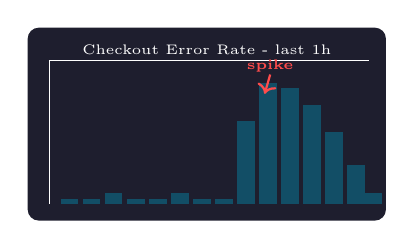
\begin{tikzpicture}[scale=0.7]
        % mock grafana chart
        \fill[codebg, rounded corners=4pt] (0,0) rectangle (6.5,3.5);
        \node[color=white!70, font=\tiny] at (3.25,3.1) {Checkout Error Rate - last 1h};
        \draw[color=white!20] (0.4,0.3) -- (0.4,2.9) -- (6.2,2.9);
        \foreach \x/\y in {
          0.6/0.4, 1.0/0.4, 1.4/0.5, 1.8/0.4,
          2.2/0.4, 2.6/0.5, 3.0/0.4, 3.4/0.4,
          3.8/1.8, 4.2/2.5, 4.6/2.4, 5.0/2.1,
          5.4/1.6, 5.8/1.0, 6.1/0.5}
          \fill[docblue] (\x,0.3) rectangle (\x+0.32,\y);
        \node[color=red!70, font=\tiny\bfseries] at (4.4,2.8) {spike};
        \draw[->, color=red!70, line width=0.8pt] (4.4,2.65) -- (4.3,2.3);
      \end{tikzpicture}

    \column{0.46\textwidth}
      \textbf{What the JSON says}

      \vspace{0.4em}
      \lstset{style=dark, language=JSON}
      \begin{lstlisting}
"event": "checkout_submit_failed",
"httpStatus": 500,
"k6": {
  "errorRate": 0.27,
  "checks": {
    "submit button visible": true,
    "checkout 2xx": false
  }
}
      \end{lstlisting}

      \vspace{0.4em}
      \small Button was there. API wasn't. 27\% of users hit this.
  \end{columns}
\end{frame}

\begin{frame}[fragile]{Step 2 - \texttt{/plan}}
  \begin{columns}[T]
    \column{0.42\textwidth}
      Type in Claude Code:

      \vspace{0.4em}
      \cmdbox{/plan}

      \vspace{0.8em}
      Planner reads:\\
      - \texttt{checkout\_error.json}\\
      - \texttt{tests/seed.spec.ts}\\
      - \texttt{app/public/index.html}

      \vspace{0.8em}
      Writes:\\
      \texttt{specs/anomaly-repro.md}

      \vspace{0.8em}
      \small Every selector verified against the live DOM before the spec is committed to disk.

    \column{0.54\textwidth}
      Output in \texttt{specs/anomaly-repro.md}:

      \lstset{style=dark}
      \begin{lstlisting}[language={}]
## Steps
1. Open the checkout page
2. Confirm session banner -> Ada Lovelace
3. Fill name, email, address, postal
4. Select Standard shipping
5. Select Credit Card
6. Click Submit payment

## Selector Map
payment-button:   [data-testid="payment-button"]
checkout-message: [data-testid="checkout-message"]

## Acceptance Criteria
- Assert success banner on happy path
- Test must fail with 500 - no masking
      \end{lstlisting}
  \end{columns}
\end{frame}

\begin{frame}[fragile]{Step 3 - \texttt{/generate}}
  \begin{columns}[T]
    \column{0.42\textwidth}
      Type in Claude Code:

      \vspace{0.4em}
      \cmdbox{/generate}

      \vspace{0.8em}
      Generator reads:\\
      - \texttt{specs/anomaly-repro.md}\\
      - validates DOM selectors

      \vspace{0.8em}
      Writes:\\
      \texttt{tests/generate/anomaly.spec.ts}

      \vspace{0.8em}
      Then run:

      \lstset{style=dark}
      \begin{lstlisting}[language=bash]
npm run test:generated
      \end{lstlisting}

      \vspace{0.4em}
      {\color{docgreen}\faCheckCircle}\quad 1 passed

    \column{0.54\textwidth}
      Also verify the failure mode:

      \lstset{style=dark}
      \begin{lstlisting}[language=bash]
CHECKOUT_FORCE_500=1 \
  npm run test:generated
      \end{lstlisting}

      \vspace{0.2em}
      {\color{red!70}\faTimes}\quad Test fails with:

      \begin{lstlisting}[language={}]
Received: "Checkout error
Upstream payment authorization failed."
Expected: "Payment submitted"
      \end{lstlisting}

      \vspace{0.4em}
      \begin{exampleblock}{\small Key insight}
        \small A test that passes under \texttt{FORCE\_500} is broken. The generator must write honest assertions.
      \end{exampleblock}
  \end{columns}
\end{frame}

\begin{frame}[fragile]{Step 4 - Simulate Drift, then \texttt{/heal}}
  \begin{columns}[T]
    \column{0.46\textwidth}
      \textbf{1. Break a selector in the DOM}

      \lstset{style=dark, language=TypeScript}
      \begin{lstlisting}
// app/public/index.html (before)
data-testid="payment-button"

// app/public/index.html (after - drift)
data-testid="pay-now-button"
      \end{lstlisting}

      \vspace{0.4em}
      \textbf{2. Run the test}

      \begin{lstlisting}[language=bash]
npm run test:generated
      \end{lstlisting}

      {\color{red!70}\faTimes}\quad Fails: \texttt{payment-button} not found

    \column{0.50\textwidth}
      \textbf{3.} Type \cmdbox{/heal}

      \vspace{0.6em}
      Healer diagnoses: locator drift (not a defect).
      Applies minimum repair:

      \begin{lstlisting}
- getByTestId('payment-button')
+ getByTestId('pay-now-button')
      \end{lstlisting}

      \vspace{0.4em}
      \textbf{4.} Re-run:

      \begin{lstlisting}[language=bash]
npm run test:generated
      \end{lstlisting}

      {\color{docgreen}\faCheckCircle}\quad 1 passed

      \vspace{0.6em}
      \small If instead the form is \textit{removed}: \texttt{test.skip()} + escalation. Healer stops.
  \end{columns}
\end{frame}

%% ══════════════════════════════════════════════════════════════
\section{04 \quad The Bigger Picture}
%% ══════════════════════════════════════════════════════════════

\begin{frame}{QA Engineers as Orchestrators}
  \begin{columns}[T]
    \column{0.48\textwidth}
      \textbf{The old model}

      \vspace{0.5em}
      QA engineer = test script author

      \vspace{0.4em}
      \begin{itemize}
        \setlength\itemsep{0.4em}
        \item Write selectors by hand
        \item Fix locators after each refactor
        \item Copy-paste AI output into test files
        \item Maintain a growing suite of brittle specs
      \end{itemize}

    \column{0.48\textwidth}
      \textbf{The emerging model}

      \vspace{0.5em}
      QA engineer = quality system orchestrator

      \vspace{0.4em}
      \begin{itemize}
        \setlength\itemsep{0.4em}
        \item Define what agents can and cannot do
        \item Write the telemetry-to-spec contract
        \item Set guardrails that protect business logic
        \item Review escalations and approve structural changes
      \end{itemize}
  \end{columns}

  \vspace{1em}
  \begin{exampleblock}{}
    \centering
    The focus shifts from \textit{writing tests} to \textit{designing systems that generate and maintain tests}.
  \end{exampleblock}
\end{frame}

\begin{frame}{What Makes This Production-Safe}
  \begin{columns}[T]
    \column{0.48\textwidth}
      \textbf{Grounding prevents hallucination}

      \vspace{0.4em}
      The seed test is the reference. Agents verify against the live DOM. Plans that cannot be grounded do not ship.

      \vspace{0.8em}
      \textbf{Spec as source of truth}

      \vspace{0.4em}
      Every test traces back to a Markdown spec. Every spec traces back to a telemetry event. The chain is auditable.

    \column{0.48\textwidth}
      \textbf{Guardrails prevent green lies}

      \vspace{0.4em}
      The Healer cannot remove assertions. A skipped test with an escalation message is the only safe alternative to a repair it cannot make.

      \vspace{0.8em}
      \textbf{Human approval gates}

      \vspace{0.4em}
      Deep structural changes require a human. The loop amplifies engineering judgment - it does not replace it.
  \end{columns}
\end{frame}

\begin{frame}{What Comes Next}
  \begin{columns}[T]
    \column{0.48\textwidth}
      \textbf{Near term}

      \vspace{0.5em}
      \begin{itemize}
        \setlength\itemsep{0.4em}
        \item Connect to real APM (Datadog, Tempo, Sentry)
        \item Run the Healer as a CI step after test failure
        \item Multi-incident parallel planning
        \item Visual regression in the seed baseline
      \end{itemize}

    \column{0.48\textwidth}
      \textbf{Further out}

      \vspace{0.5em}
      \begin{itemize}
        \setlength\itemsep{0.4em}
        \item Agents that explore the app and propose new specs
        \item Healer that opens a PR instead of editing in place
        \item Cross-service telemetry correlation
        \item QA coverage maps driven by user session replays
      \end{itemize}
  \end{columns}

  \vspace{1em}
  \begin{block}{The key question is no longer}
    \centering "Can AI write tests?" - it is "What does a QA system\\look like when the feedback loop is continuous and autonomous?"
  \end{block}
\end{frame}

%% ── Takeaways ────────────────────────────────────────────────
\begin{frame}{Key Takeaways}
  \begin{enumerate}
    \setlength\itemsep{0.8em}
    \item \textbf{Telemetry is a test specification waiting to be read.}\\
          \small Production signals carry enough context to drive Planner agents - no manual translation needed.

    \item \textbf{MCP makes agents actionable, not just generative.}\\
          \small Without file access and tool execution, LLMs write suggestions. With MCP, they write tests.

    \item \textbf{Guardrails are not constraints - they are the product.}\\
          \small Defining what an agent can and cannot do is the engineering work. The agent executes it.

    \item \textbf{The Healer's job is to know when to stop.}\\
          \small A \texttt{.skip} with an honest escalation is more valuable than a green build that masks a defect.

    \item \textbf{QA engineers become orchestrators of quality systems.}\\
          \small The shift is from writing tests to designing the loop that generates and maintains them.
  \end{enumerate}
\end{frame}

%% ── Q&A ──────────────────────────────────────────────────────
{
\setbeamercolor{background canvas}{bg=docblue}
\begin{frame}[plain]
  \vspace{2cm}
  \begin{center}
    {\color{white}\Huge Q \& A}\\[1em]
    {\color{white!70}\large Thank you}\\[2em]
    {\color{white!60}\small
      Repository: \texttt{playwright-agentic-testing-wmf-2026}\\[0.4em]
      Tutorial: \texttt{http://127.0.0.1:3002}\\[0.4em]
      Slash commands: \texttt{/plan} \textperiodcentered{} \texttt{/generate} \textperiodcentered{} \texttt{/heal} \textperiodcentered{} \texttt{/demo}
    }
  \end{center}
\end{frame}
}

%% ─────────────────────────────────────────────────────────────
\end{document}
%% ─────────────────────────────────────────────────────────────